\chapter{Evaluation}

[TODO compare the speedup we get to a perfect $T_1$ to $T_\infty$ speedup]

If we overlay the results from the previous sections, we can compare the performance of the different algorithms presented thus far. 

\begin{figure}[!htbp]
\begin{centering}
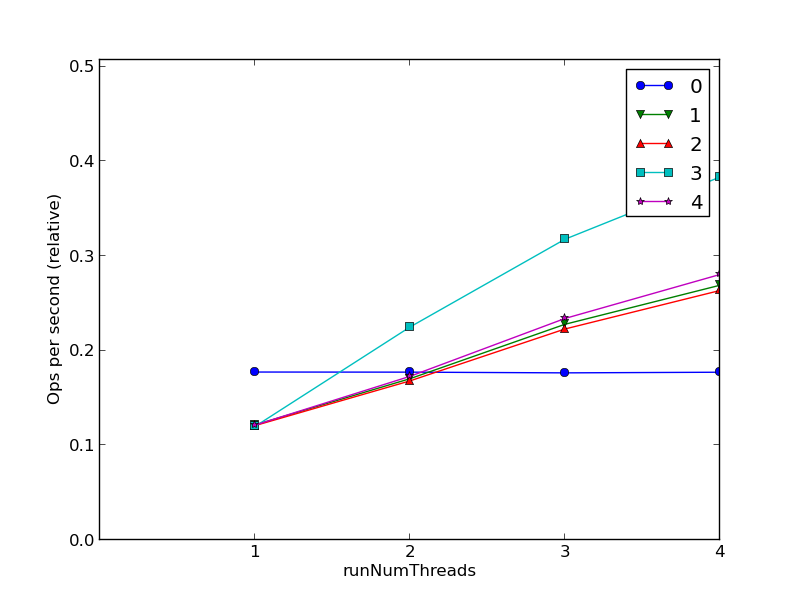
\includegraphics[width=0.8\textwidth]{{{images/threads-xper5-sherlock-all-2}}}
\end{centering}
\caption{Throughput with 1 to 4 threads on Sherlock, All Methods, XPERIENCE domain}
\label{fig:thread-sax-2}
\end{figure}

Looking at throughput on Sherlock using the XPERIENCE domain in Figure~\ref{fig:thread-sax-2}, we can see that all the algorithms have a certain cost above the baseline single-threaded method. Method 3, the work-stealing queue, becomes better than baseline starting from 2 threads, and remains better than the other algorithms by a comfortable margin. The other algorithms still manage to scale linearly, becoming better than the baseline by 3 threads, and are very close to each other in terms of performance.

\begin{figure}[!htbp]
\begin{centering}
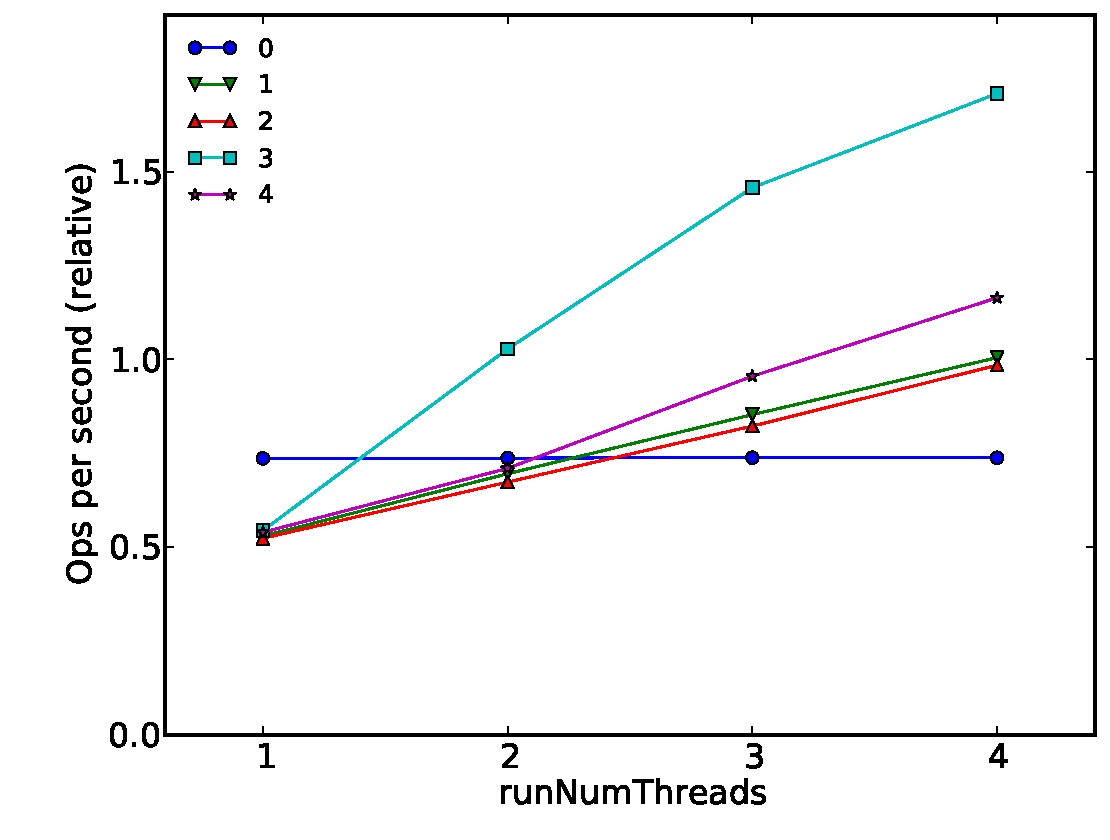
\includegraphics[width=0.8\textwidth]{{{images/threads-log3-sherlock-all-2}}}
\end{centering}
\caption{Throughput with 1 to 4 threads on Sherlock, All Methods, Logistics domain}
\label{fig:thread-sal-2}
\end{figure}

The results on the Logistics domain in Figure~\ref{fig:thread-sal-2} are very similar, although on this domain Method 4, the global queue, manages to do better than Methods 1 \& 2. The work-stealing queue remains comfortably faster than all the others.

\begin{figure}[!htbp]
\begin{centering}
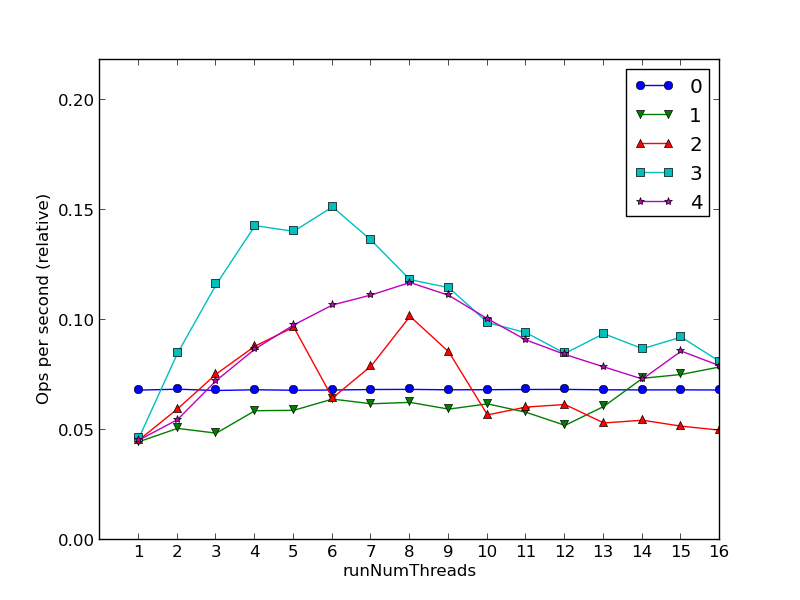
\includegraphics[width=0.8\textwidth]{{{images/threads-xper5-catzilla.inf.ed.ac.uk-all-2}}}
\end{centering}
\caption{Throughput with 1 to 4 threads on Catzilla, All Methods, XPERIENCE domain}
\label{fig:thread-cax-2}
\end{figure}

On Catzilla, the different algorithms differentiate themselves a little further. In Figure~\ref{fig:thread-cax-2}, we can see Method 3, the work-stealing queue remains much faster. Here, Method 1 struggles to ever climb past the baseline single-threaded performance, suggesting that thread creation overhead may be much higher on this machine. Method 2, the blocking queues, and Method 4, the global queue, start very close but the global queue eventually overtakes the blocking queue in terms of performance.

\begin{figure}[!htbp]
\begin{centering}
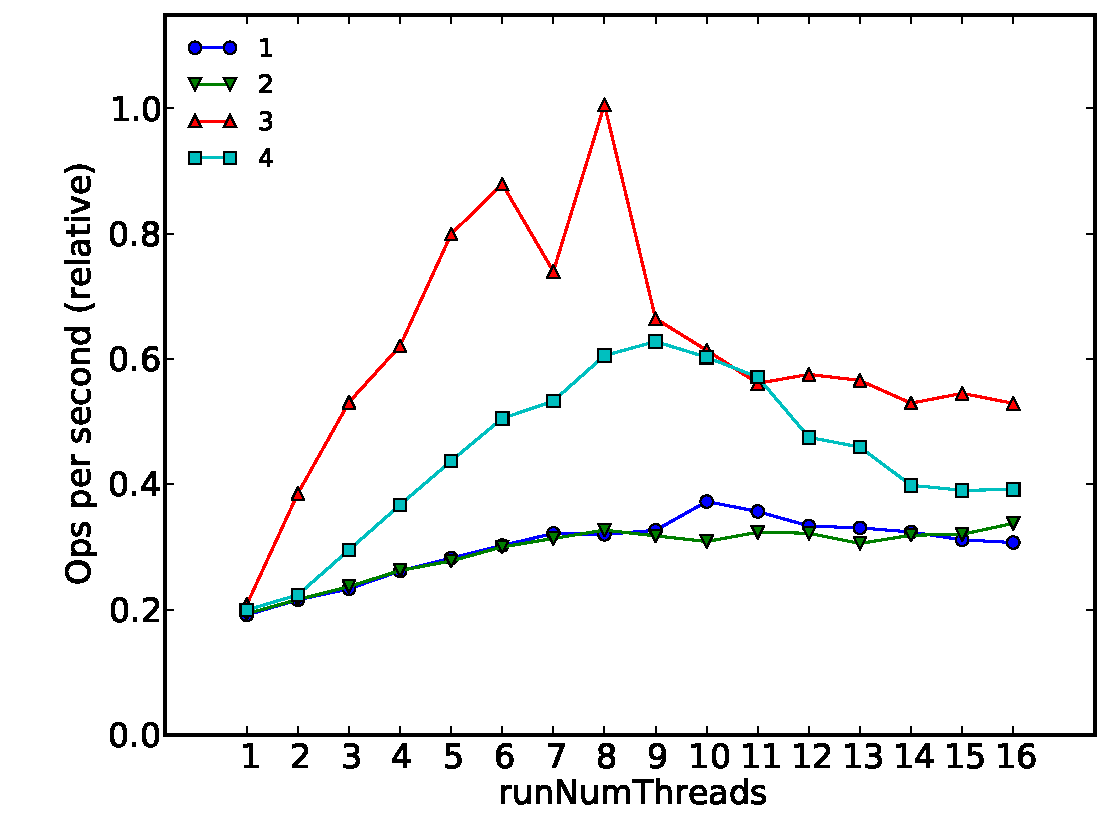
\includegraphics[width=0.8\textwidth]{{{images/threads-log3-catzilla.inf.ed.ac.uk-all-2}}}
\end{centering}
\caption{Throughput with 1 to 4 threads on Catzilla, All Methods, Logistics domain}
\label{fig:thread-cal-2}
\end{figure}

[TODO method0 on catzilla results missing for Logistics domain!]

In Figure~\ref{fig:thread-cal-2}, we see the same results for the Logistics domain. Here Method 2, the blocking queue, performs even worse relative to Method 4, the global queue. The global queue scales well, but the work-stealing queue remains by far the fastest.

[TODO cachegrind/memory analysis]

In general, we have seen that the Logistics domain seems to scale up to a larger number of threads than the XPERIENCE domain, and we have seen that a possible cause of scaling difficulties comes from cache contention during memory allocation. Another compelling piece of evidence comes from graphing the number of new explanation generated by each existing explanation, when a new observation is processed.

\begin{figure}[!htbp]
\begin{centering}
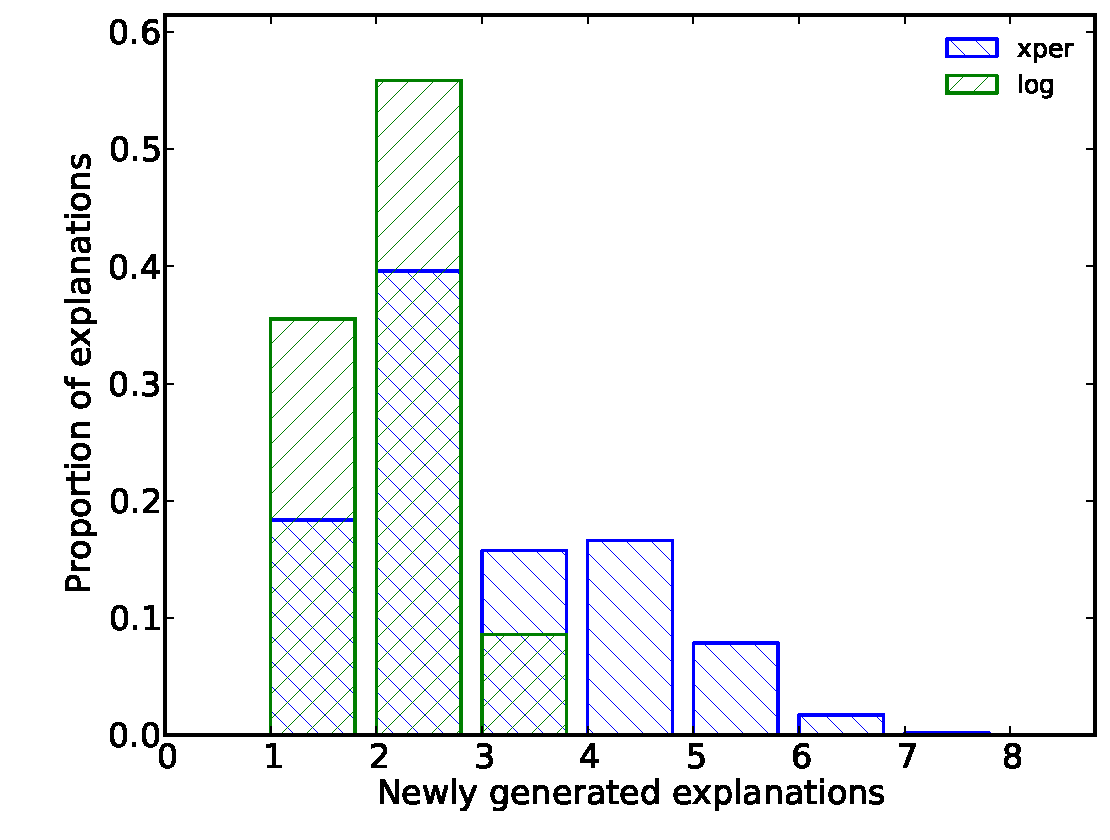
\includegraphics[width=0.8\textwidth]{{{images/histogram}}}
\end{centering}
\caption{Number of generated explanations from each previous explanation, for both domains}
\label{fig:hist}
\end{figure}

In Figure~\ref{fig:hist}, we see that each new observation in the Logistics domain typically produces only one or two explanations to replace it. However in the XPERIENCE domain, a significant proportion of explanations will produce 3 to 5 new ones to replace it. This would imply an increased rate of memory allocation and more cache contention.